% Picar el capitulo entre Implementacion y Experimentos
% Añadir un p\'arrafo al final de Implementacion de como se utilza el nuevo sistema
\chapter{AutoGOAL Multiobjetivo}\label{chapter:implementation}
AutoGOAL \brackcite{estevez2020solving} es un sistema AutoML Heterog\'eneo modular y f\'acilmente extensible. Modela su espacio de b\'usqueda utilizando Gram\'aticas Probabil\'istica  Libre del Contexto (PCFG) \brackcite{megane2021probabilistic}, una extensi\'on de las Gram\'aticas Libres del Contexto al asignar a cada producci\'on una probabilidad. Con el fin de dirigir la b\'usqueda utiliza Evoluci\'on Gramatical Probabil\'istca (\textit{Probabilistic Grammatical Evolution}, PGE) \brackcite{megane2021probabilistic}, una modificaci\'on de Evoluci\'on Gramatical (\textit{Grammatical Evolution}) \brackcite{o2001grammatical}
%basada en Algoritmos de Estimaci\'on de Distribuci\'on (EDAs)
para ser usada con PCFG.

PGE est\'a basado en Algoritmos de Estimaci\'on de Distribuci\'on (EDAs) \brackcite{larranaga2001estimation} una t\'ecnica evolutiva que remplaza las operaciones de mutaci\'on y cruce por un muestreado sobre las probabilidades de las producciones de PCFG. Dado una gram\'atica $G$ y una cadena $c \in G$, PGE modifica las probabilidades asociadas a cada producci\'on de $G$ para que las pr\'oximas cadenas generadas con $G$ tengan mayor probabilidad de utilizar las mismas producciones que $c$. Cuando $c$ representa el individuo m\'as aptos entonces las pr\'oximas generaciones tienen mayor probabilidad de conservar sus caracter\'isticas.
Este es un algoritmo sencillo pero efectivo que logra un balance entre exploraci\'on y explotaci\'on local haci\'endolo resistente a m\'inimos locales y a la generaci\'on de soluciones iguales.

AutoGOAL posee cualidades que lo hacen un candidato natural para la implementaci\'on de la propuesta definida en el cap\'itulo \ref{chapter:proposal}:
\begin{enumerate}
    \item Su arquitectura modular permite la adici\'on sencilla  de un nuevo optimizador. 
    \item El optimizador multiobjetivo se beneficia del algoritmo gen\'etico subyacente que utiliza AutoGOAL para modelar su espacio de b\'usqueda. 
\end{enumerate}

% Su modelaci\'on del espacio de b\'usqueda utilizando un algoritmo gen\'etico donde en cada iteraci\'on se acerca m\'as a la soluci\'on \'optima combina con el MOEA de la propuesta.
% La arquitectura m\'odular de AutoGOAL junto con su espacio de de b\'usqueda modelado con algoritmos gen\'eticos lo hacen un candidato natural para la implementaci\'on de la propuesta definida en el cap\'itulo \ref{chapter:proposal}. 

\section{Implementaci\'on}

\begin{figure}[ht]
    \centering
    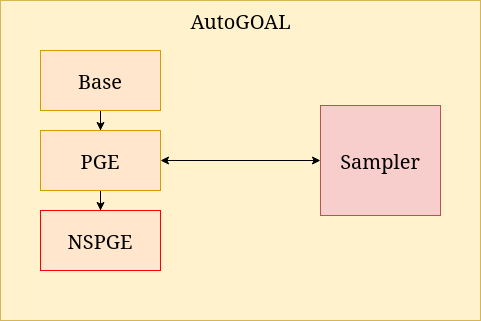
\includegraphics[scale=0.6]{Pictures/autogoal_impl.png}
    \caption{Diagrama general}
    \label{impl:fig:general_diagram}
\end{figure}


AutoGOAL representa la PCFG utilizada para modelar su espacio de decisi\'on a trav\'es de un grafo ac\'iclico dirigido (DAG) donde cada nodo representa una posible cadena de la gram\'atica y sus aristas apuntan a todas las posibles cadenas a las que se puede expandir sustituyendo un No Terminal por una producci\'on 
%de la Gram\'atica
correspondiente. Cuando una cadena se encuentra completamente expandida, i.e. compuesta por solo s\'imbolos terminales, se tiene una soluci\'on v\'alida del sistema. 

Cada arista del DAG se inicializa con una probabilidad igual a todas todas las aristas que salen de su mismo nodo tal que la suma de sus probabilidades sea 1. Un camino se escoge utilizando una variable uniforme donde su valor determina la arista a seleccionar.
Una vez que se tiene un individuo apto AutoGOAL aplica PGE sobre el grafo actualizando las probabilidades de todas las aristas seg\'un el camino utilizado por dicho individuo. Esta operaci\'on se realiza sobre los $k$ individuos m\'as aptos de la poblaci\'on generada. %PGE en AutoGOAL utiliza una lista de los $k$ individuos m\'as aptos para actualizar el grafo.
% Cuando se tiene un individuo apto la manera de AutoGOAL de conservar sus ``genes'' es aplicando PGE sobre las aristas que conforman el camino que condujo a esa soluci\'on. M\'as especificamente, la implementaci\'on de AutoGOAL de PGE dado $n$ individuos, son evaluados respecto a un criterio de evaluaci\'on $f$ y se crea una lista de las $k$ mejores soluciones (encabezada por la m\'as apta) y las aristas de las probabilidades se actualizan de acuerdo a estas soluciones. 

\subsection{NSPGE}
NSPGE (\textit{Nondominated Sorting using PGE}), un algoritmo de b\'usqueda basado en la propuesta del cap\'itulo \ref{chapter:proposal}, define una nueva ordenaci\'on sobre las soluciones generadas por AutoGOAL. Se define como una clase que hereda directamente de PGE con el objetivo de extender la l\'ogica encargada de seleccionar los mejores individuos de acuerdo a m\'ultiples m\'etricas y reutilizar la l\'ogica de muestreado que utiliza PGE para actualizar la gram\'atica. PGE define su l\'ogica de selecci\'on de individuos dentro del m\'etodo \textit{\_indices\_of\_the\_fittest\_}, el cual NSPGE sobreescribe.

\subsubsection{Ciclo Principal}
La redefinici\'on \textit{\_indices\_of\_the\_fittest\_} incluye las dos etapas de ordenaci\'on definidas por NSGA-II \brackcite{deb2002fast}. Dado $n$ soluciones se utiliza \textit{Non Dominated Sorting} para dividirlas en frentes de distinto rango (\ref{proposal:def:rank_front}). Luego se itera sobre los frentes en orden ascendente de acuerdo a su \'indice de dominaci\'on. En cada iteraci\'on a\~naden todos los elementos de un frente siempre que el conjunto respuesta tenga capacidad. Cuando haya  mayor cantidad de elementos en un frente que posiciones disponibles en el conjunto soluci\'on se aplica \textit{Crowding Distance} sobre el frente y se seleccionan los individuos de mayor distancia.

\begin{lstlisting}[caption=Nueva ordenaci\'on, language=Python]
def _indices_of_fittest(self, fns: List[List[float]]):
  # Se ordenan todas las soluciones segun su orden
  # de dominacion
  fronts = self.non_dominated_sort(fns)
  indices = []
  k = int(self._selection * len(fns))

  # Se forma el conjunto solucion
  for front in fronts:
    if len(indices) + len(front) <= k:
      indices.extend(front)
    else:
      # Cuando solo el frente no puede utilizarse
      # completo se aplica crowding distance
      indices.extend(
          sorted(
              front,
              key=lambda i: -self.crowding_distance(fns, front, i)
          )[: k - len(indices)]
      )
      break
  return indices
\end{lstlisting}

\subsubsection{Non Dominated Sorting}
Se conforma por dos pasos l\'ogicos fundamentales:
\begin{enumerate}
    \item Se verifica todo par de soluciones $x, y$ encontradas y se aplica $x \prec y$ con el objetivo de calcular el \'indice de dominaci\'on de cada soluci\'on. Adem\'as se construye un DAG conformado por las soluciones donde existe una arista entre las soluciones $x$ y $y$ si $x \prec y$. La ra\'iz de dicho DAG est\'a conformado por las soluciones que nadie domina.
    \item Se recorre DAG utilizando una versi\'on de BFS (\textit{Breadth First Search}) partiendo por las soluciones que tienen \'indice de dominaci\'on 0. Todas las soluciones visitadas se les reduce el \'indice de dominaci\'on en uno. Si llega a 0 se a\~nade al frente de Pareto que se est\'a formando. Luego se comienza el proceso nuevamente partiendo por las soluciones a las cuales su \'indice se redujo a 0.
\end{enumerate}

\begin{lstlisting}[caption=Selecci\'on seg\'un \'indice de dominaci\'on, language=Python]
def non_dominated_sort(self, scores: List[List[float]]):
  # fronts almacena los frentes 
  #(i.e. fronts[i] es el frente de rango i)
  fronts: List[List[int]] = [[]]

  # domination_rank en i indica la cantidad de soluciones
  # que dominan a la solucion i
  domination_rank = [0] * len(scores)

  # dominated_scores en i alamacena las soluciones dominadas
  # por la solucion i
  dominated_scores = [list() for _ in scores]

  # revisa todo par de soluciones y se establece
  # quien dominan a quien
  for i, score_i in enumerate(scores):
    for j, score_j in enumerate(scores):
      if self._improves(score_i, score_j):
          dominated_scores[i].append(j)
      elif self._improves(score_j, score_i):
          domination_rank[i] += 1
    if domination_rank[i] == 0:
       fronts[0].append(i)

  # de acuerdo a la informacion sobre quienes
  # se dominan, forma todos los frentes
  front_rank = 0
  while len(fronts[front_rank]) > 0:
    next_front = []
    for i in fronts[front_rank]:
      for dominated in dominated_scores[i]:
        domination_rank[dominated] -= 1
        if domination_rank[dominated] == 0:
          next_front.append(dominated)
    front_rank += 1
    fronts.append(next_front)

  return fronts[:-1]
\end{lstlisting}

\subsubsection{Crowding Distance Sorting}
Se sigue la idea del algoritmo propuesto en (\ref{proposal:alg:cd}). Dado $m$ m\'etricas a evaluar se realizan $m$ iteraciones, donde en cada una se ordena un frente de rango $k$ de acuerdo a la m\'etrica $m_i$. Las soluciones que con respecto a la m\'etrica $m_i$ tienen el m\'inimo y mayor valor se les asigna distancia infinita y luego se calculan los valores intermedios. Las componentes de los vectores soluci\'on se normalizan antes de ejecutar \textit{Crowding Distance} aplicando \textit{feature scaling} para llevar todos los valores al rango [0, 1].

\begin{lstlisting}[caption=Selecci\'on seg\'un estimaci\'on de densidad, language=Python]
def crowding_distance(
    self, scores: List[List[float]], front: List[int], index: int
) -> float:
  # Crowding distance usa los vectores normalizados.
  # Se aplica feature scaling para llevar cada
  # componente de los vectores al rango [0, 1]
  scaled_scores = feature_scaling(scores)

  crowding_distances: List[float] = [0 for _ in scores]
  for m in range(len(self._maximize)):
    # Se ordena de acuerdo a la metrica m
    front = sorted(front, key=lambda x: scores[x][m])

    # Se establecen los extremos como infinitos
    crowding_distances[front[0]] = math.inf
    crowding_distances[front[-1]] = math.inf

    # Valores de todas las soluciones con respecto a m 
    m_values = [scaled_scores[i][m] for i in front]
    scale: float = max(m_values) - min(m_values)
    if scale == 0:
      scale = 1
    for i in range(1, len(front) - 1):
      crowding_distances[i] += (
        scaled_scores[front[i + 1]][m] - scaled_scores[front[i - 1]][m]
      ) / scale

  return crowding_distances[index]
\end{lstlisting}

\subsection{Adaptaciones a AutoGOAL}
Adem\'as de la adici\'on de la clase NSPGE, la infraestructura interna de AutoGOAL fue actualizada para permitir la optimizaci\'on multiobjetivo:
\begin{itemize}
    \item La clase AutoML espera el conjunto de mejores soluciones encontradas y sus evaluaciones en vez de la mejor.
    \item El algoritmo base que explora el espacio de b\'usqueda utiliza el concepto de \textit{Pareto dominaci\'on} para comparar las soluciones.
    \item En cada  iteraci\'on se almacena los $k$ mejores individuos encontrados y no el m\'as apto respecto a una sola m\'etrica.
    \item El algoritmo se detiene cuando no encuentra ninguna soluci\'on mejor que alguna de las $k$ mejores.
    \item La respuesta del optimizador es el frente de rango $0$ tras aplicar \textit{Non Dominated Sorting} a las $k$ mejores soluciones encontradas durante todo el ciclo de ejecuci\'on. Idealmente corresponde con una aproximaci\'on del frente de Pareto.
\end{itemize}

\section{Aplicaci\'on de AutoGOAL Multiobjetivo}
AutoGOAL Multiobjetivo mantiene la misma interfaz que AutoGOAL. Para utilizar esta nueva ordenaci\'on se necesita  se\~nalar el algoritmo de b\'usqueda a utilizar con el par\'ametro \textbf{search\_algorithm}. Adem\'as es necesario definir una m\'etrica que retorne 2 o m\'as valores en \textbf{score\_metric} y especificar por cada una si se desea maximizar o minimizar utilizando el par\'ametro  \textbf{maximize}. 

\begin{lstlisting}[caption=Uso de AutoGOAL con multiobjetivo, language=Python]
from autogoal.datasets import cars
from autogoal.kb import (
  MatrixContinuousDense,
  Supervised,
  VectorCategorical
)
from autogoal.ml import AutoML
from autogoal.search import NSPESearch

automl = AutoML(
    input=(MatrixContinuousDense, Supervised[VectorCategorical]),
    output=VectorCategorical,
    search_algorithm=NSPESearch, # Algoritmo de Busqueda
    score_metric=accuracy_vs_time, # Metrica de varios criterios
    maximize=(True, True), # Componentes de la metrica a maximizar
)

# Entrena el modelo
x, y = cars.load()
automl.fit(x, y)

# Imprime todas las soluciones encontradas
print(automl.best_pipeline_) 
\end{lstlisting}

\subsection{M\'etricas}
Las m\'etricas se utilizan para evaluar el rendimiento de las soluciones generadas por AutoGOAL.
La definici\'on de m\'etricas multiobjetivo  es similar a como se definen en AutoGOAL est\'andar con la diferencia de que estas retornan tuplas de elementos como se muestra en (\ref{impl:metrics}). 

Es \'util poder definir todas las m\'etricas dentro de una funci\'on pues permite mayor control sobre el espacio objetivo ya que se pueden definir relaciones entre estas. La segunda m\'etrica definida, \textit{acc\_vs\_train\_time\_better}, es superior a la primera porque desestima las soluciones que tienen exactitud 0.

\begin{lstlisting}[caption=Ejemplo de m\'etrica: \textit{accuracy} contra tiempo, language=Python, label=impl:metrics]
from time import time
import autogoal.ml.metrics as metrics
import math

def acc_vs_train_time(*args, **kwargs):
    t1 = time()
    acc = metrics.accuracy(*args, **kwargs)
    t2 = time()
    return [acc, t1 - t2]

def acc_vs_train_time_better(*args, **kwargs):
    t1 = time()
    acc = metrics.accuracy(*args, **kwargs)
    t2 = time()
    return [acc, t1 - t2] if acc > 0 else [-math.inf, -math.inf]
\end{lstlisting}
